\thispagestyle{duongvaotoanhocnone}
\pagestyle{duongvaotoanhoc}
\everymath{\color{duongvaotoanhoc}}
\graphicspath{{../duongvaotoanhoc/pic/}}
\blfootnote{$^1$\color{duongvaotoanhoc}Viện Toán học.}
\begingroup
\AddToShipoutPicture*{\put(0,616){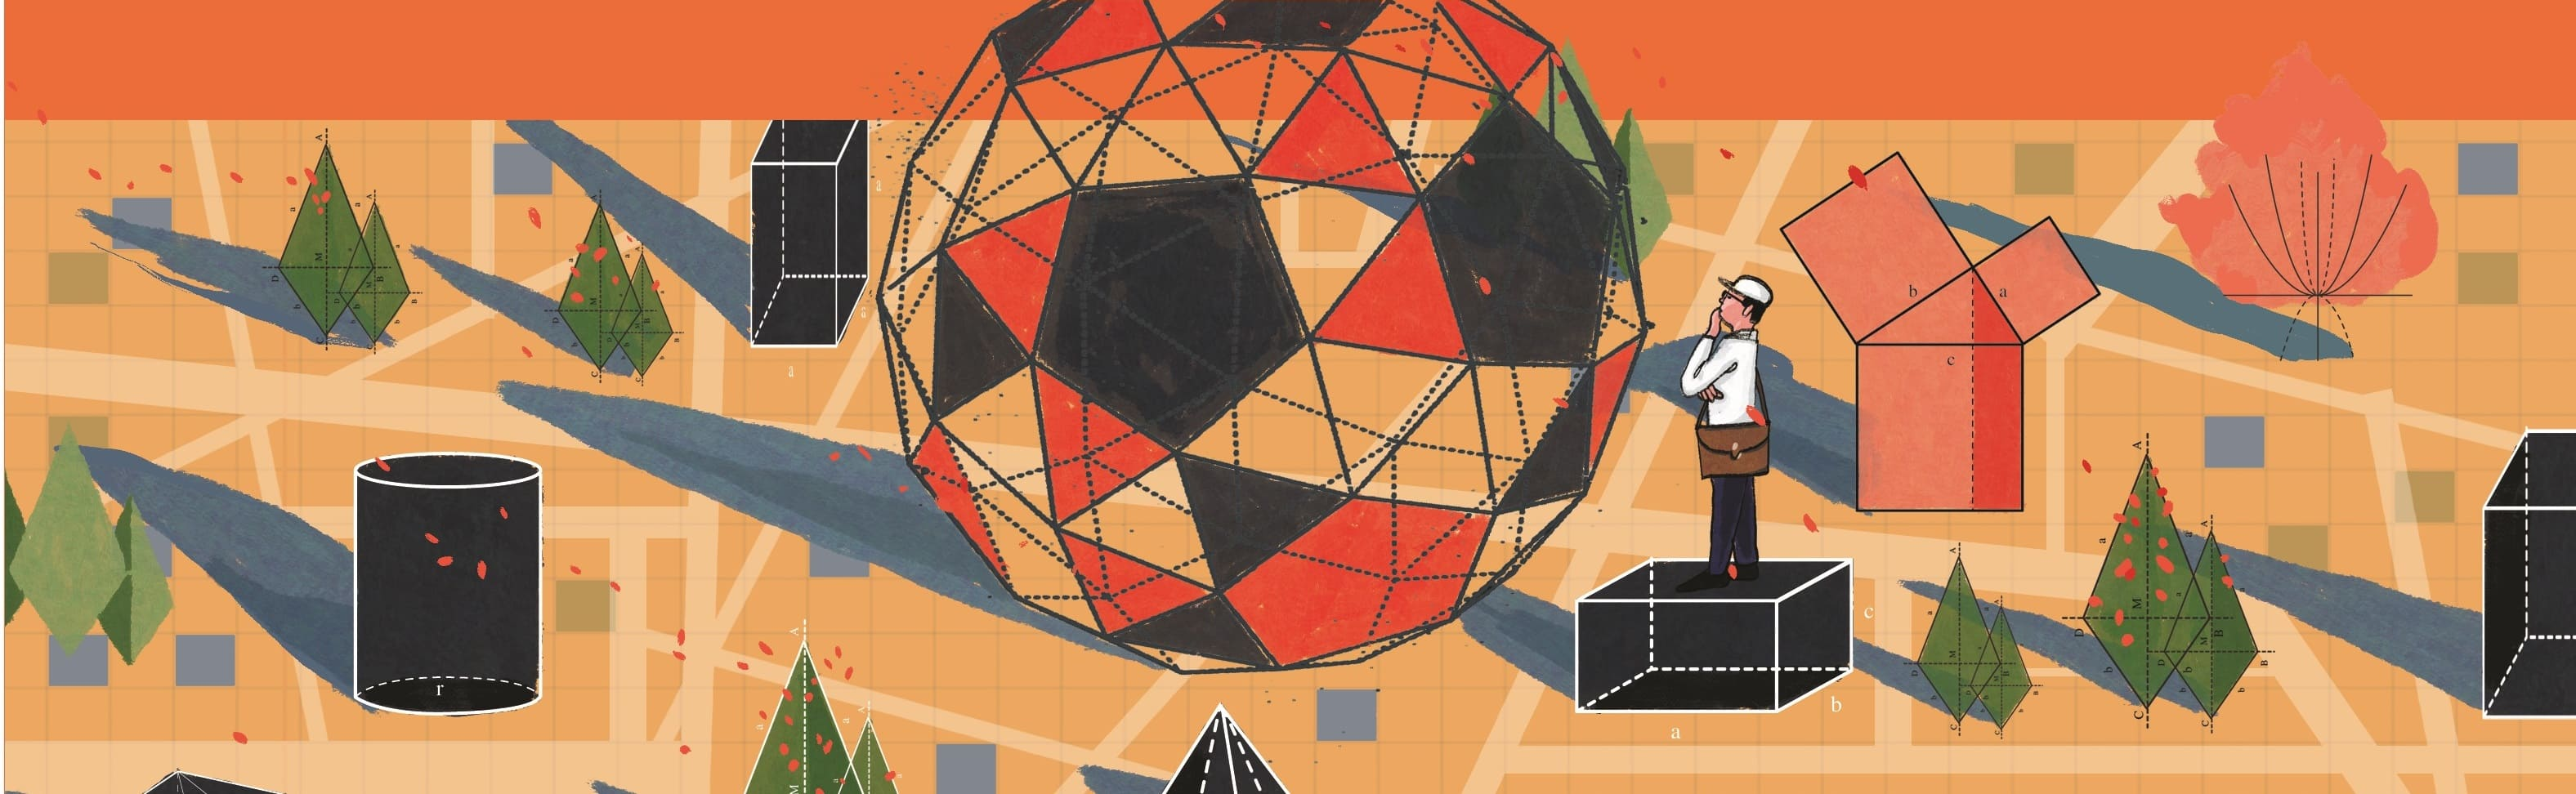
\includegraphics[width=19.3cm]{../bannerduongvao}}}
\AddToShipoutPicture*{\put(168,553){
\includegraphics[scale=1]{../tieude.pdf}}}
\centering
\endgroup
\vspace*{154pt}

\begin{multicols}{2}	
	\begin{center}
		\begin{tikzpicture}[line cap=round,line join=round,>=triangle 45,x=1cm,y=1cm]
			\begin{axis}[
				x=1cm,y=1cm,
				axis lines=middle,
				ymajorgrids=true,
				xmajorgrids=true,
				xmin=-1.7883986831624292,
				xmax=2.4523577489207637,
				ymin=-2.3395044710908626,
				ymax=2.8687249112773965,
				xtick={-1.5,-1,...,2},
				ytick={-2,-1.5,...,2.5},]
				\clip(-1.7883986831624292,-2.3395044710908626) rectangle (2.4523577489207637,2.8687249112773965);
				
				%WARNING: PGF/Tikz and Gnuplot don't support implicit curves
				%Rather try PSTricks export
				%Cannot draw -1*y^2+1*x^3
				
			\end{axis}
		\end{tikzpicture}
	\end{center}

\end{multicols}